\documentclass[compress, aspectratio=149]{beamer}
\usepackage[english]{babel}

\usepackage{amsthm}
\usepackage{mathtools}
\usepackage{physics}
\usepackage{calligra}
\usepackage{csquotes}
\usepackage{tensor}
\usepackage[thicklines]{cancel}
\usepackage{tcolorbox}
\usepackage{pstricks}

\usepackage{multirow}
\usepackage{multicol}
\usepackage{bigdelim}

\usepackage{tabularx}
\usepackage{tikz}
\usepackage{mathtools}
\usepackage{amsmath,amssymb}

%\usepackage[font=footnotesize,labelfont={color=orange,bf}]{caption}
\usepackage{graphicx}

\usepackage[absolute,overlay]{textpos}
%\usepackage[texcoord,grid,gridcolor=red!10,subgridcolor=green!10,gridunit=pt]{eso-pic}

\usepackage{xparse}
\NewDocumentCommand{\framecolorbox}{oommm}
    {% #1 = width (optional)
    % #2 = inner alignment (optional)
    % #3 = frame color
    % #4 = background color
    % #5 = text
    \IfValueTF{#1}
    {%
    \IfValueTF{#2}
     {\fcolorbox{#3}{#4}{\makebox[#1][#2]{#5}}}
     {\fcolorbox{#3}{#4}{\makebox[#1]{#5}}}%
    }
    {\fcolorbox{#3}{#4}{#5}}%
    }

\usepackage[natbib=true,backend=biber,style=apa, sorting=nty, citestyle=authoryear-comp]{biblatex} %Custom bibliography
    \addbibresource{bib.bib} %Load references

\AtBeginBibliography{\footnotesize}

\DeclareMathAlphabet{\mathcalligra}{T1}{calligra}{m}{n}
\DeclareFontShape{T1}{calligra}{m}{n}{<->s*[2.2]callig15}{}
\newcommand{\scriptr}{\mathcalligra{r}\,}
\newcommand{\boldscriptr}{\pmb{\mathcalligra{r}}\,}
\def\rc{\scriptr}
\def\brc{\boldscriptr}
\def\hrc{\hat\brc}
\newcommand{\ie}{\emph{i.e.}} %id est
\newcommand{\eg}{\emph{e.g.}} %exempli gratia
\newcommand{\rtd}[1]{\ensuremath{\left\lfloor #1 \right\rfloor}}
\newcommand{\dirac}[1]{\ensuremath{\delta \left( #1 \right)}}
\newcommand{\diract}[1]{\ensuremath{\delta^3 \left( #1 \right)}}
\newcommand{\e}{\ensuremath{\epsilon_0}}
\newcommand{\m}{\ensuremath{\mu_0}}
\newcommand{\V}{\ensuremath{\mathcal{V}}}
\newcommand{\prnt}[1]{\ensuremath{\left(#1\right)}} %parentheses
\newcommand{\colch}[1]{\ensuremath{\left[#1\right]}} %square brackets
\newcommand{\chave}[1]{\ensuremath{\left\{#1\right\}}}  %curly brackets

\useoutertheme{infolines}
\useinnertheme{rectangles}
\usefonttheme{professionalfonts}


\definecolor{orange}{HTML}{f28165}
\definecolor{gray}{HTML}{303030}
\definecolor{yellow}{HTML}{f0be52}
\definecolor{lightorange}{HTML}{f19e58}
\definecolor{myblue}{cmyk}{1,.72,0,.38}
\definecolor{aliceblue}{rgb}{0.94, 0.97, 1.0}

\renewcommand{\CancelColor}{\color{orange}}

\makeatletter
\newcommand{\mybox}[1]{%
  \setbox0=\hbox{#1}%
  \setlength{\@tempdima}{\dimexpr\wd0+13pt}%
  \begin{tcolorbox}[colback=orange,colframe=orange,boxrule=0.5pt,arc=4pt,
      left=6pt,right=6pt,top=6pt,bottom=6pt,boxsep=0pt,width=\@tempdima]
    \textcolor{white}{#1}
  \end{tcolorbox}
}
\makeatother

\usecolortheme[named=orange]{structure}
\usecolortheme{sidebartab}
\usecolortheme{orchid}
\usecolortheme{whale}
\setbeamercolor{alerted text}{fg=yellow}
\setbeamercolor{block title alerted}{bg=alerted text.fg!90!black}
\setbeamercolor{block title example}{bg=lightorange!60!black}
\setbeamercolor{background canvas}{bg=gray}
\setbeamercolor{normal text}{bg=gray,fg=white}
\setbeamercolor{subsection in head/foot}{bg=white, fg=gray}


\setbeamertemplate{blocks}[rectangle]
\setbeamercovered{dynamic}

\setbeamertemplate{caption}[numbered]

\setbeamertemplate{section page}
{
	\begin{centering}
		\begin{beamercolorbox}[sep=27pt,center]{part title}
			\usebeamerfont{section title}\insertsection\par
			\usebeamerfont{subsection title}\insertsubsection\par
		\end{beamercolorbox}
	\end{centering}
}

\addtobeamertemplate{navigation symbols}{}{ \hspace{1em}    \usebeamerfont{footline}%
    \insertframenumber / \inserttotalframenumber }
\setbeamertemplate{navigation symbols}{}

%\beamer@compresstrue
\defbeamertemplate*{headline}{smoothbars theme}{%
  \begin{beamercolorbox}[ht=2.125ex,dp=3.150ex]{section in head/foot}
  \insertnavigation{\paperwidth}
  \end{beamercolorbox}%

  \begin{beamercolorbox}[ht=2.125ex,dp=1.125ex,%
  leftskip=.3cm,rightskip=.3cm plus1fil]{subsection in head/foot}
  \usebeamerfont{subsection in head/foot}\insertsubsectionhead
  \end{beamercolorbox}%
}

\setbeamertemplate{subsection page}
{
	\begin{centering}
		\begin{beamercolorbox}[sep=12pt,center]{part title}
			\usebeamerfont{subsection title}\insertsubsection\par
		\end{beamercolorbox}
	\end{centering}
}

\newcommand{\hlight}[1]{\colorbox{violet!50}{#1}}
\newcommand{\hlighta}[1]{\colorbox{red!50}{#1}}

\newcommand{\boxorange}[1]{
\begin{center}
\fcolorbox{orange}{gray}{
\begin{minipage}{0.95\textwidth}
#1
\end{minipage}
}
\end{center}
}

\newcommand{\boxgrey}[1]{
\begin{center}
\fcolorbox{black!85!white}{lightgray!35!white}{
\begin{minipage}{0.8\textwidth}
#1
\end{minipage}
}
\end{center}
}

\setlength{\abovecaptionskip}{5pt plus 3pt minus 2pt}

% Block colors
\colorlet{orangeTitleBlockColor}{orange}
\colorlet{orangeBlockColor}{orange!25!gray}
\colorlet{blockTitleTextColor}{gray}
\colorlet{blockBodyTextColor}{white}

\setbeamertemplate{blocks}[rectangle]

\setbeamercolor*{block title}{
  fg=blockTitleTextColor,
  bg=orangeTitleBlockColor}
\setbeamercolor*{block body}{
  fg=blockBodyTextColor,
  bg=orangeBlockColor}
  
\setbeamerfont{block title}{size={}}

\AtBeginEnvironment{block}{%
  \setbeamercolor{itemize item}{fg=orangeTitleBlockColor!70}}
  

\title[\cite{roussille2021central}]{The Central Role of the Ask Gap}
\subtitle{\large in Gender Pay Inequality}
\author{Nina Roussille}
\institute[Sai Zhang]{Presented by: Sai Zhang}
\date{March 23, 2023}

\begin{document}

\bgroup
\setbeamertemplate{navigation symbols}{}
\makeatother
\bgroup

\setbeamertemplate{footline}
        {
      \leavevmode%
      \hbox{%
      \begin{beamercolorbox}[wd=.2\paperwidth,ht=2.25ex,dp=1ex,left]{author in head/foot}%
        \usebeamerfont{author in head/foot}\hspace*{2em} \insertshortinstitute
      \end{beamercolorbox}%
      \begin{beamercolorbox}[wd=.6\paperwidth,ht=2.25ex,dp=1ex,center]{title in head/foot}%
        \usebeamerfont{title in head/foot}\insertshorttitle
      \end{beamercolorbox}%
      \begin{beamercolorbox}[wd=.2\paperwidth,ht=2.25ex,dp=1ex,right]{date in head/foot}%
        \usebeamerfont{date in head/foot}\insertshortdate{}\hspace*{2em}

    %#turning the next line into a comment, erases the frame numbers
        %\insertframenumber{} / \inserttotalframenumber\hspace*{2ex} 

      \end{beamercolorbox}}%
      \vskip0pt%
    }
    
    \frame{\titlepage}
    
    \setbeamertemplate{footline}
        {
      \leavevmode%
      \hbox{%
      \begin{beamercolorbox}[wd=.2\paperwidth,ht=2.25ex,dp=1ex,left]{author in head/foot}%
        \usebeamerfont{author in head/foot}\hspace*{2em}\insertshortinstitute
      \end{beamercolorbox}%
      \begin{beamercolorbox}[wd=.6\paperwidth,ht=2.25ex,dp=1ex,center]{title in head/foot}%
        \usebeamerfont{title in head/foot}\insertshorttitle
      \end{beamercolorbox}%
      \begin{beamercolorbox}[wd=.2\paperwidth,ht=2.25ex,dp=1ex,right]{date in head/foot}%
        \usebeamerfont{date in head/foot}\insertframenumber{}\hspace*{2em}

    %#turning the next line into a comment, erases the frame numbers
        %\insertframenumber{} / \inserttotalframenumber\hspace*{2ex} 

      \end{beamercolorbox}}%
      \vskip0pt%
    }
    \setcounter{framenumber}{0}
    
    \begin{frame}{Outline}
        \tableofcontents
    \end{frame}
    
    \setbeamercovered{invisible}
    \section{Introduction}
\frame{\sectionpage}
\begin{frame}{Theoretical Inspiration}
    \uncover<+->{How to hold politicians accountable?} \uncover<+->{Provide {\textcolor<8>{orange} {\textbf<8>{information}}}!}
    
    \begin{itemize}
        \item[-]<+-> Accountability is closely linked to voters' information access {\scriptsize \citep{przeworski1999democracy}}
        \item[-]<+-> Improving information availability has an impact {\scriptsize \citep{alesina2007bureaucrats,besley2006handcuffs,majumdar2004politics,persson2000political}}
    \end{itemize}
    
    \vspace{10pt}
    \uncover<+->{How influential is the information?}
    \begin{itemize}
        \item[-]<+-> Acquiring: \textcolor<8>{orange}{\textbf<8>{Endogenous}} characteristics matter {\scriptsize \citep{downs1957economic}}
        \item[-]<+-> Interpreting: \textcolor<8>{orange}{\textbf<8>{Beliefs}} and biases matter {\scriptsize \citep{rabin1998psychology}} 
    \end{itemize}
    
\end{frame}

\begin{frame}{Empirical Uniqueness}
\textbf{\color{orange}\underline{Question}:}
\begin{quote}
    The effects of the disclosure of local governmental corruption practices on the electoral outcomes of incumbents in Brazil’s municipal elections
\end{quote}

\begin{enumerate}
    \item<2-> Endogeneity: \uncover<3->{municipal governments are \textbf{\color{orange}randomly} selected to be audited}
    \only<4>{\begin{itemize}
        \item \textbf{\color{orange}Which} municipalities get audited 
        \item \textbf{\color{orange}When} the municipalities get audited
    \end{itemize}}
    
    \item<5-> Beliefs: The \textbf{\textcolor{orange}{incumbent}}'s revealed corruption level serves as a shock
    
    \item<6-> Information: 
    \uncover<6->{
    \begin{itemize}
        \item measure of corruption\only<7>{: \textbf{\color{orange}objectively} constructed from audit reports}
        \item dissemination of information\only<7>{: the presence of {\textbf{\color{orange}local media}} {\scriptsize(radio, in particular)}}
    \end{itemize}
    }
\end{enumerate}

\end{frame}

\begin{frame}{Preview of Results}
    \begin{enumerate}
        \item<1-> Information matters:
        \begin{itemize}
            \item<2-> Among municipalities where 2 corrupt violations were reported, the audit policy treatment reduced the incumbent's reelection likelihood by \textbf{\color{orange}7 percentage points (17\%)}
            \item<3-> Treatment effect raises to \textbf{\color{orange}14 percentage points} when 3 corrupt violations were reported 
        \end{itemize}
        \item<4-> Media is a dissemination channel: 
        \begin{itemize}
            \item<5-> Punishment is amplified: Among municipalities \textbf{\color{orange}with 1 radio station} where 2 corrupt violations were reported, the audit policy treatment reduced the incumbent's reelection likelihood by \textbf{\color{orange}11 percentage points}
            \item<6-> It also rewards:  Among municipalities \textbf{\color{orange}with 1 radio station} where \textbf{\color{orange}0} corrupt violations were reported,  the audit policy treatment \textbf{\color{orange}increased} the incumbent's reelection likelihood by \textbf{\color{orange}17 percentage points}
        \end{itemize}
 
    \end{enumerate}
\end{frame}

\begin{frame}{Contribution}
\begin{enumerate}
    \item<2-> An \textcolor<3->{orange}{\textbf<3->{objective measure}} of corruption
    \only<3-4>{\begin{itemize}
        \item<3-4> Previously, only charges/accusations were used 
        
        {\scriptsize\citet{peters1980effects} for US House, \citet{changgolden} for Italy}
        \item<4> Objective measures of corruption became more prevalent 
        
        {\scriptsize\citet{golden2005proposal} for Italy}
    \end{itemize}}
    
    \item<5-> Empirical support for the \textbf<6->{\textcolor<6->{orange}{value of information}}
    \only<6-7>{
    \begin{itemize}
        \item<6-7> on political selection {\scriptsize \citep{besley2005political,besleypande2005political}}
        \item<7> complementing previous studies on government responsiveness {\scriptsize \citep{besley2002political,di2003role,reinikka2005fighting,yang2008integrity}}
    \end{itemize}}
    
    \item<8-> Exploring the \textcolor<9->{orange}{\textbf<9->{role of media}}
    
    \only<9-10>{\scriptsize
    cross-country study \citep{brunetti2003free} 
    
    newspapers \citep{besley2002political,gentzkow2006rise} 
    
    \textbf<10>{\textcolor<10>{orange}{radio \citep{stromberg2004radio}}}
    }
    
    \item<11-> \textbf{\color{orange}Evaluation} of anti-corruption programs
    
    \only<12>{\scriptsize parallel to the RCT setting of \citet{olken2007monitoring}}
\end{enumerate}
    
\end{frame}


    
    \section{Context}
    
\frame{\sectionpage}

\begin{frame}{Hired.com: The Market}
    \begin{itemize}
        \item<+-> high-stake recruitment
        \begin{itemize}
            \item[-] most candidates are looking for \textit{\underline{full-time jobs}}: \textcolor{frenchlilac!45!white}{\textbf{96.9\%}} 
            \item[-] \textit{\underline{highly educated}} candidates: \textcolor{frenchlilac!45!white}{\textbf{97.6\%}} bachelor {\tiny and above}, \textcolor{frenchlilac!45!white}{\textbf{41.4\%}} master {\tiny and above}
            \item[-] \textit{\underline{highly paid}} jobs: average annual salary \textcolor{frenchlilac!45!white}{\textbf{\$119,548}}
        \end{itemize} 
        \item<+-> mostly tech industry
        \begin{itemize}
            \item[-] economic significance of tech labor market
            \item[-] substantial gender imbalance: \textcolor{frenchlilac!45!white}{\textbf{20.8\% female}} on Hired.com
        \end{itemize}
    \end{itemize}
\end{frame}

\begin{frame}{Hiring Process on Hired.com}
    \begin{columns}[T]
        \begin{column}{0.3\textwidth}
            \begin{block}{\small \centering \textbf{Ask} Salary}
                \begin{figure}
                    \centering
                    
\includegraphics[width = 0.95 \textwidth]{images/hireprocess1.png}
                \end{figure}
            \end{block}
        \end{column}

        \begin{column}{0.3\textwidth}
            \begin{block}{\small \centering \textbf{Bid} Salary}
                \begin{figure}
                    \centering
                    
\includegraphics[width = 0.95 \textwidth]{images/hireprocess2.png}
                \end{figure}
            \end{block}
        \end{column}

        \begin{column}{0.3\textwidth}
            \begin{block}{\small \centering \textbf{Final} Salary}
                \begin{figure}
                    \centering
                    
\includegraphics[width = 0.95 \textwidth]{images/hireprocess3.png}
                \end{figure}
            \end{block}
        \end{column}
    \end{columns}
\end{frame}

\begin{frame}{Supply Side: Jobseekers' Profile}
    \begin{figure}
        \centering
        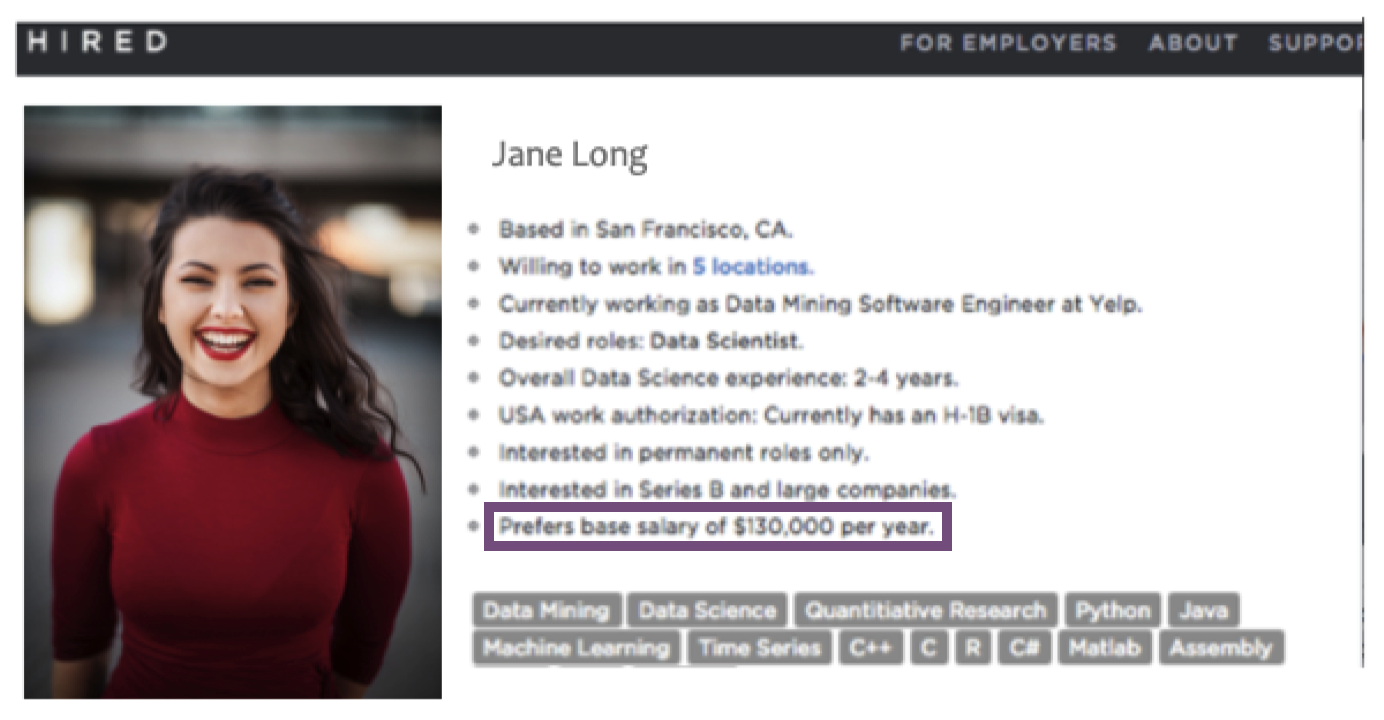
\includegraphics[height = 0.75 \textheight]{images/jobseeker.png}
    \end{figure}
\end{frame}

\begin{frame}{Demand Side: Employers' Interview Request}
    \begin{figure}
        \centering
        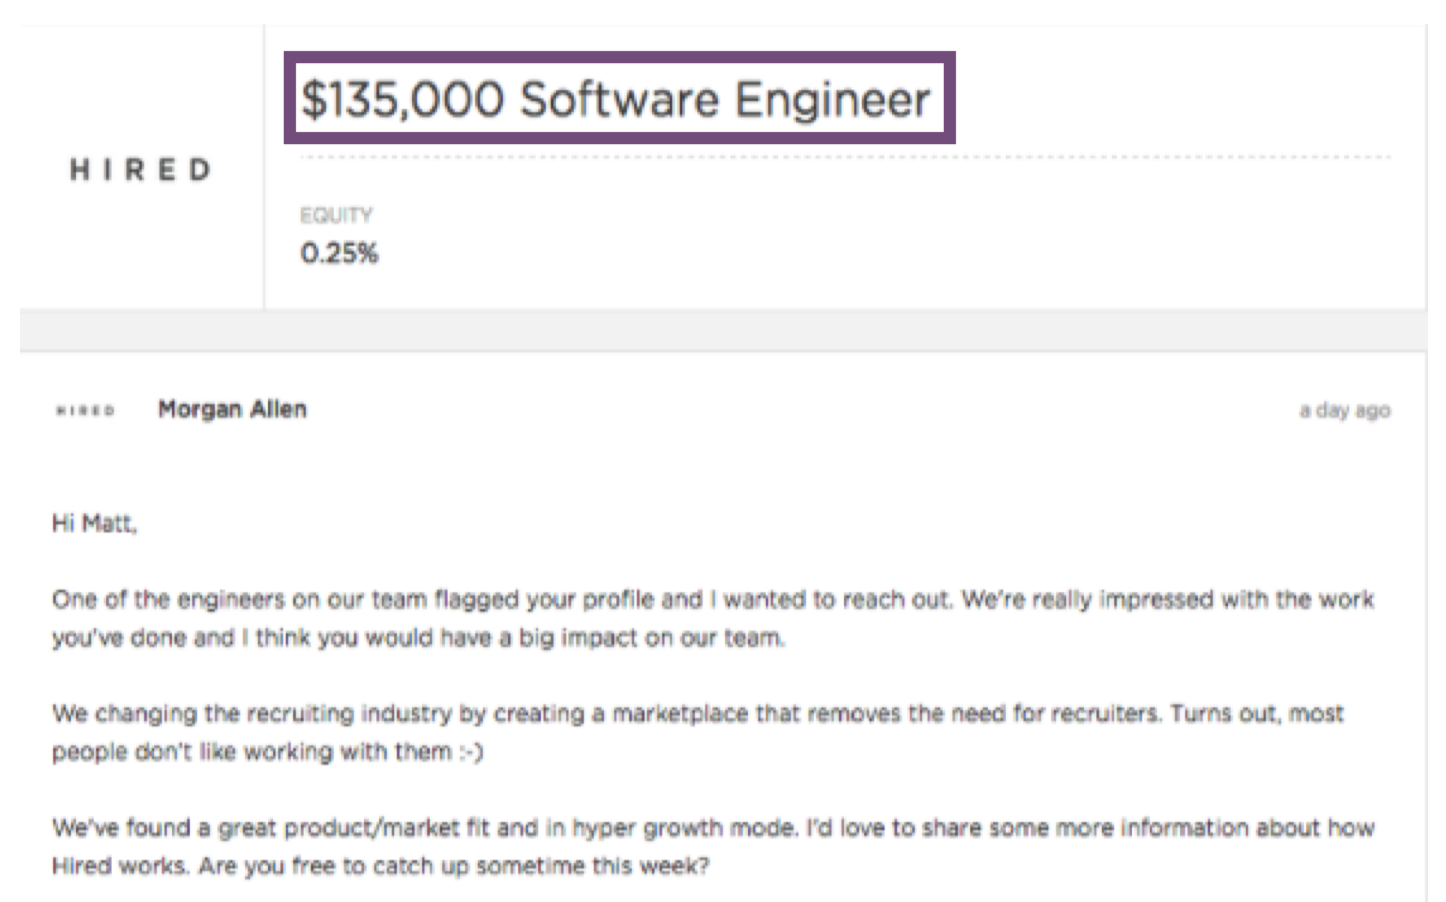
\includegraphics[height = 0.75 \textheight]{images/employer.png}
    \end{figure}
\end{frame}

\begin{frame}{Recap: Hiring Process on Hired.com}
    \begin{figure}
        \centering
        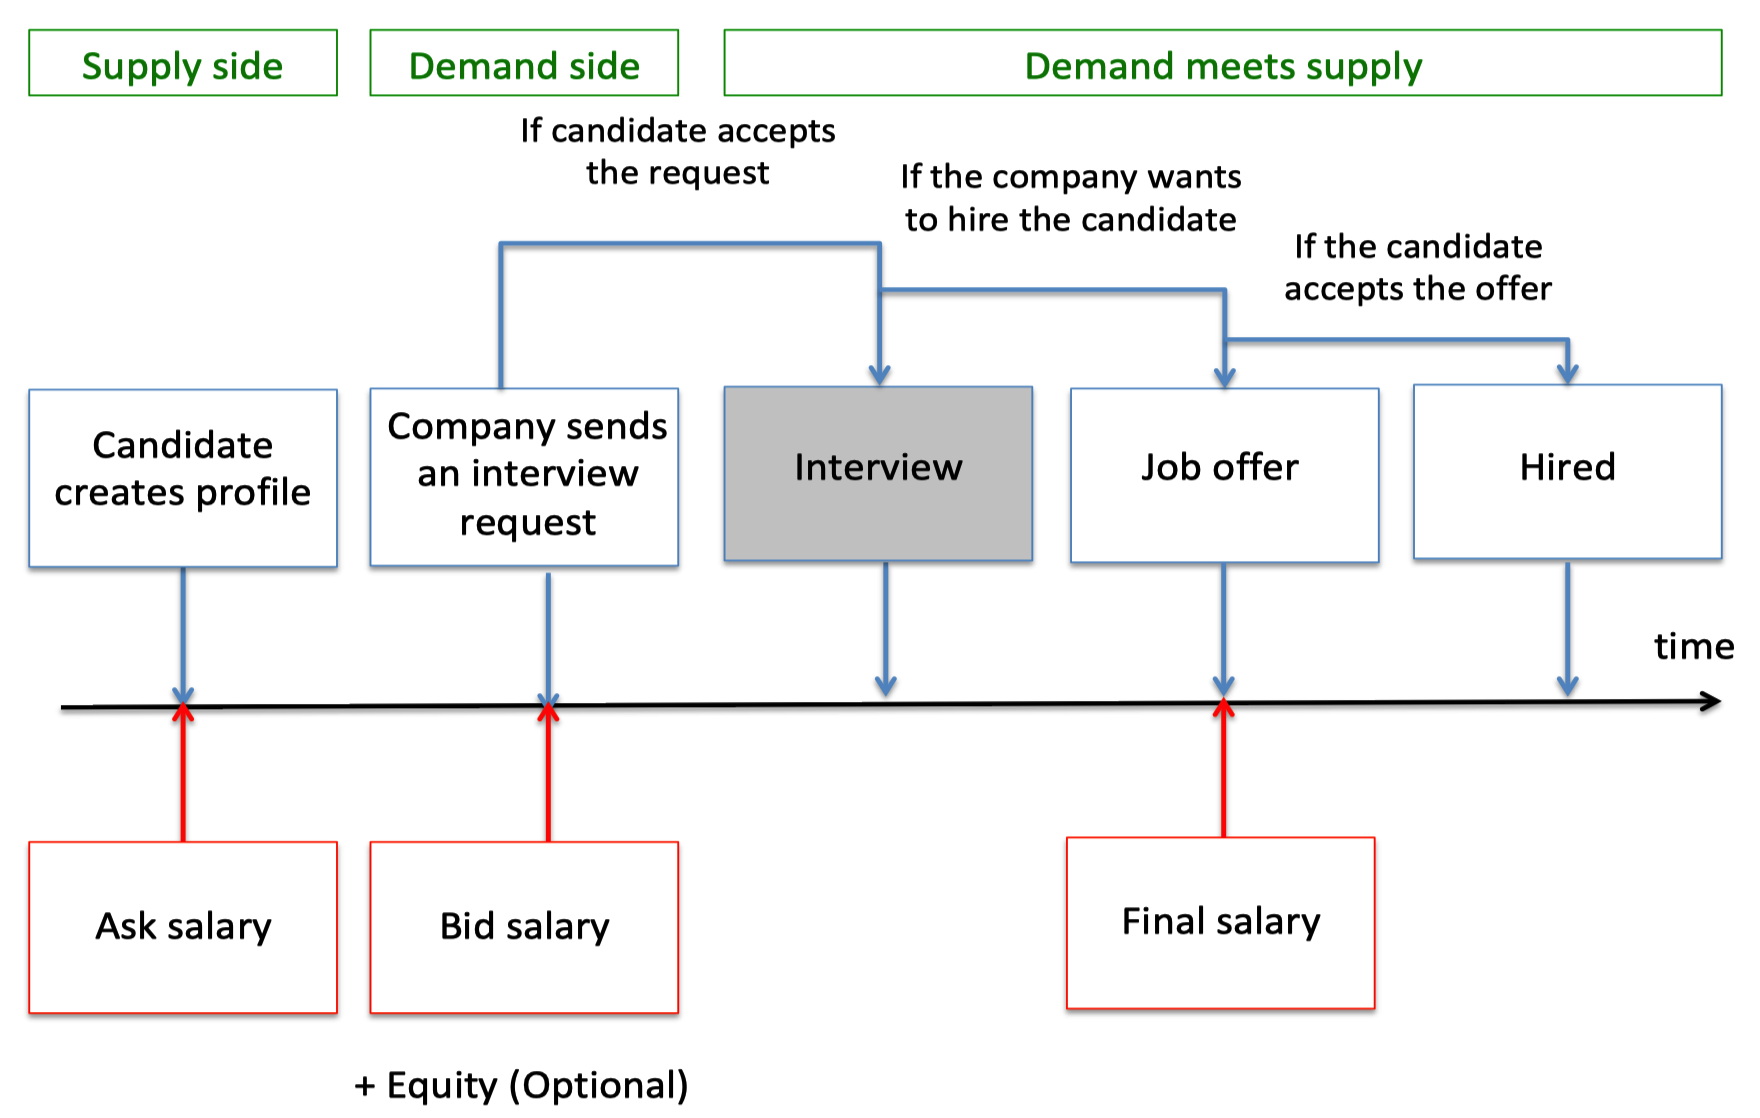
\includegraphics[height = 0.7 \textheight]{images/hiringflow.png}
    \end{figure}
\end{frame}

    
    \section{Data}

 \frame{\sectionpage}

    \begin{frame}{Data}
        \begin{itemize}
            \item {\color{mygreen}\underline{\textit{Non-farm sectors}}}: Annual Survey of Industries (ASI)
            
            \hfill {\small 10 waves from 2000-2001 to 2009-2010 fiscal years, firm-level data} % all registered manufacturing 50 workers more, random 1/3 of registered with >10 workers
            \item {\color{mygreen}\underline{\textit{Consumption}}}: National Sample Survey (NSS) Consumer Expenditure Survey
            
            \hfill {\small 7 waves from 2003-2004 to 2011-2012}
            \item {\color{mygreen}\underline{\textit{Wages and Employment}}}: NSS Employment and Unemployment Survey
            \item {\color{mygreen}\underline{\textit{Agricultural}}}: Ministry of Agriculture
            
            \hfill {\small unbalanced panel (2000-2010, crop-by-year) and other district-level measures}
        \end{itemize}
    \end{frame}

    \begin{frame}{Data: Treatment}
        \begin{itemize}
            \item<1-> {\color{mygreen}\underline{\textit{Rainfall}}}: Topical Rainfall Measuring Mission (TRMM)
            
            \hfill {\small daily rainfall measures, 0.25-by-0.25 degree grid-cell size}
            
            \hfill {\small aggregate to district-year total monsoon rainfall (Jun. to Sep.)}

            \hfill {\small nonlinearlity as Jayachandran (2006)}
            \item<2-> {\color{mygreen}\underline{\textit{NREGA}}}: NSS Employment and Unemployment Survey
            
            \hfill {\small compared with state-level statutory NREGA wages from administrative sources}
        \end{itemize}
    
    \end{frame}

 \begin{frame}{Variables: Industry}
    \begin{itemize}
        \item<1-> \underline{\textit{traded vs. non-traded classifier}}:
        \begin{itemize}
            \item[-] \citet{holmes2014alternative} Commodity Flow Survey (CFS) industry classification by \textcolor{mygreen}{\underline{transportation cost}}
            \item[-] \citet{mian2014explains} and Kothari (2014):
             \begin{itemize}
                \item[$\cdot$] \textcolor{mygreen}{\underline{geographical concentration}} of industrial production across counties
                \item[$\cdot$] degree of \textcolor{mygreen}{\underline{international trade}} 
             \end{itemize}
        \end{itemize}
        \item<2-> \underline{\textit{agricultural linkage classifier}}: upstream/downstream/non-linked industries of agriculture (MOSPI, 2004-2005) %large share of agricultural output/input
        \item<3-> \underline{\textit{financial performance indicator}}:
        \begin{itemize}
            \item[-] capital intensity
            \item[-] dependence on external finance
        \end{itemize}
    \end{itemize}

 \end{frame}

 \begin{frame}{Variables: Firm}
    \begin{itemize}
        \item<1-> \underline{\textit{firms' production}}: value of total output
        \item<1-> \underline{\textit{firms' employment}}: total number of works and total number of man-days employed
        \item<1-> \underline{\textit{daily wage}}: $\frac{\text{total compensation paid}}{\text{number of man-days}}$
    \end{itemize}

 \end{frame}



    \section{Results}

 \frame{\sectionpage}

\begin{frame}{Estimation I: Exogenous Treatment}
\only<1->{
    \small
    \begin{equation*}
        E_{ms} = \alpha + \textcolor{orange}{\beta}A_{ms} + X_{ms}\gamma + \nu_s+ \epsilon_{ms}
    \end{equation*}
}

\uncover<1->{
    \begin{table}[h!]
        \footnotesize
        \begin{center}
            \label{tab:result1}
            \begin{tabular}{lcccc}
            
            & \multicolumn{2}{c}{All incumbent mayors} & & Those ran \\
            & (1) & (2) & & (3) \\
            \hline
            Preelection audit (1/0) & \textcolor<2-3>{orange}{-0.036} & \textcolor<2-4>{orange}{0.036} & & \textcolor<2,4>{orange}{-0.059} \\
             & \textcolor<2-3>{orange}{(0.053)} & \textcolor<2-4>{orange}{(0.052)} & & \textcolor<2,4>{orange}{(0.065)}\\
             Observations & 373 & 373 &  & 263\\
             $R^2$ & 0.05 & 0.17 & & 0.22\\
             State FEs & Yes & Yes & & Yes\\
             Municipal controls & \textcolor<3>{orange}{No} & \textcolor<3>{orange}{Yes} & & Yes \\
             Mayoral controls & \textcolor<3>{orange}{No} & \textcolor<3>{orange}{Yes} & & Yes
            \end{tabular}
        \end{center}
        \end{table}

    {\footnotesize \textbf{\color{orange} Note:} Hereafter, robust standard errors are displayed in parenthesis, significant levels: 99\%(**), 95\%(*), 90\%(+).}
    }
    
\end{frame}

\begin{frame}{Estimation I: Exogenous Treatment}
    \only<1->{
    \small
    \begin{equation*}
        E_{ms} = \alpha + \textcolor{orange}{\beta}A_{ms} + X_{ms}\gamma + \nu_s+ \epsilon_{ms}
    \end{equation*}
}

\uncover<1->{
    \begin{table}[h!]
        \footnotesize
        \begin{center}
            \label{tab:result2}
            \begin{tabular}{lccccc}
            
            \multicolumn{6}{c}{Only mayors ran for reelection}\\
            \hline
            & Pr(reelection) & Vote share & Win margin & $\Delta$vote share & $\Delta$win margin \\
            & (3) & (4) & (5) & (6) & (7) \\
            \hline
            Preelection audit (1/0) & -0.059 & -0.055 & -0.020 & -0.032$^{+}$ & -0.028 \\
             & (0.065) & (0.072) & (0.027) & (0.018) & (0.027)\\
             Observations & 263 & 263 & 263 & 263 & 263\\
             $R^2$ & 0.22 & 0.16 & 0.22 & 0.39 & 0.31 \\
             State FEs & \multicolumn{5}{c}{Yes}\\
             Municipal controls  & \multicolumn{5}{c}{Yes} \\
             Mayoral controls  & \multicolumn{5}{c}{Yes}
            \end{tabular}
        \end{center}
        \end{table}

    }
\end{frame}

\begin{frame}{Estimation I: Exogenous Treatment}
    \only<1->{
    \small
    \begin{equation*}
        E_{ms} = \alpha + \textcolor{orange}{\beta}A_{ms} + X_{ms}\gamma + \nu_s+ \epsilon_{ms}
    \end{equation*}
}

Results: $\beta=0$

\vspace*{20pt}

\begin{enumerate}
    \small
    \item<2-> \textbf{\color{orange}Beliefs} matter: The effects of surprisingly low and high levels of corruption cancel each other out.
    \item<3-> \textbf{\color{orange}Media presence} matters: Information might not be so effectively disseminated.
\end{enumerate}
    
\end{frame}

\begin{frame}{Estimation II: Adding Voters' Prior Beliefs}
    \begin{figure}\label{fig3}
        \centering
        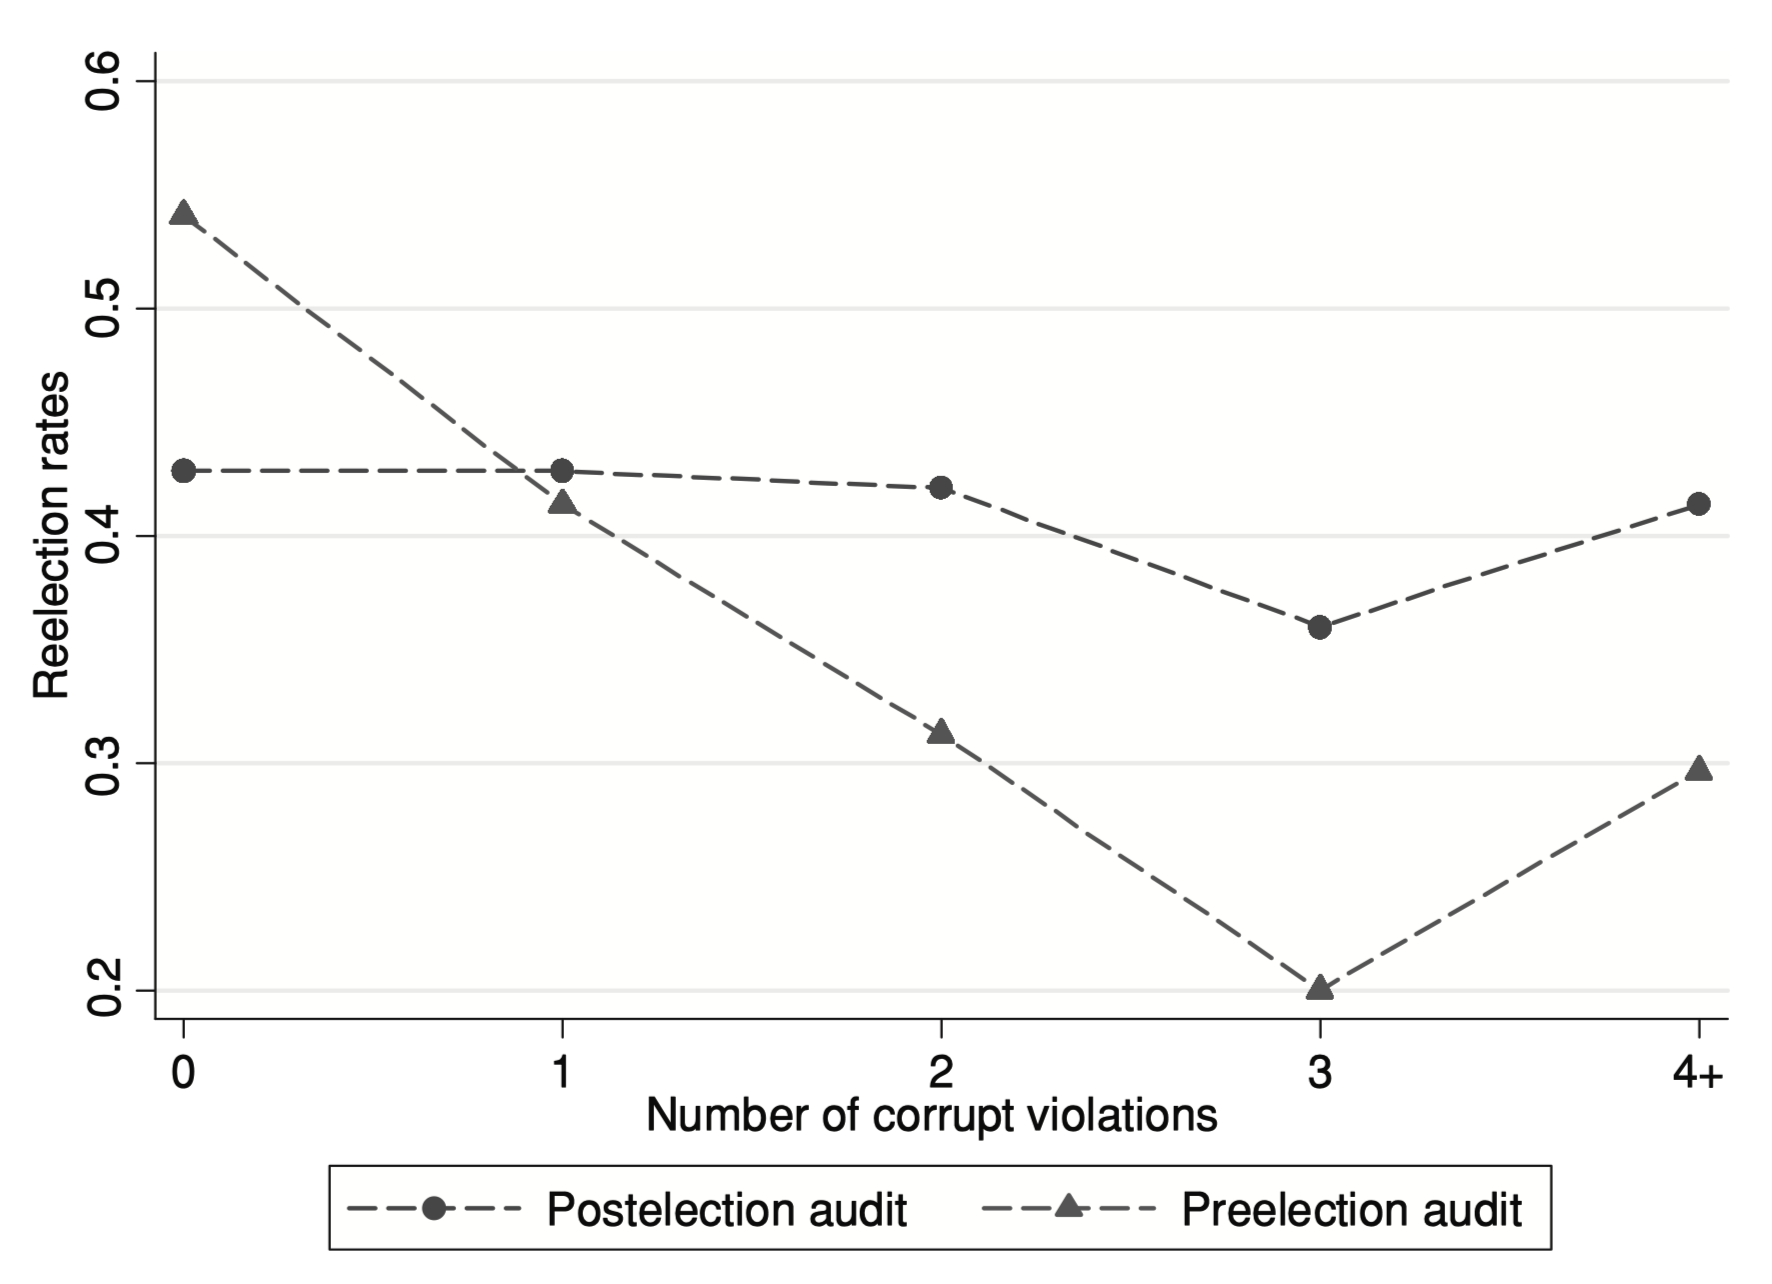
\includegraphics[height = 0.65 \textheight]{images/fig3.png}
        \caption{Descriptive evidence: Reelection Rates and Corruption Levels}
        \end{figure}
\end{frame}

\begin{frame}{Estimation II: Adding Voters' Prior Beliefs}

    \only<1>{
            \footnotesize
            \begin{align*}
                E_{ms} =& \alpha + \beta_0 C_{ms} + \beta_1 A_{ms} + \textcolor{orange}{\beta_2} \left(A_{ms}\times C_{ms}\right) + X_{ms}\gamma + \nu_s + \epsilon_{ms}
            \end{align*}
            }

    \begin{columns}

        \begin{column}{0.4\textwidth}
            \begin{figure}
            \centering
            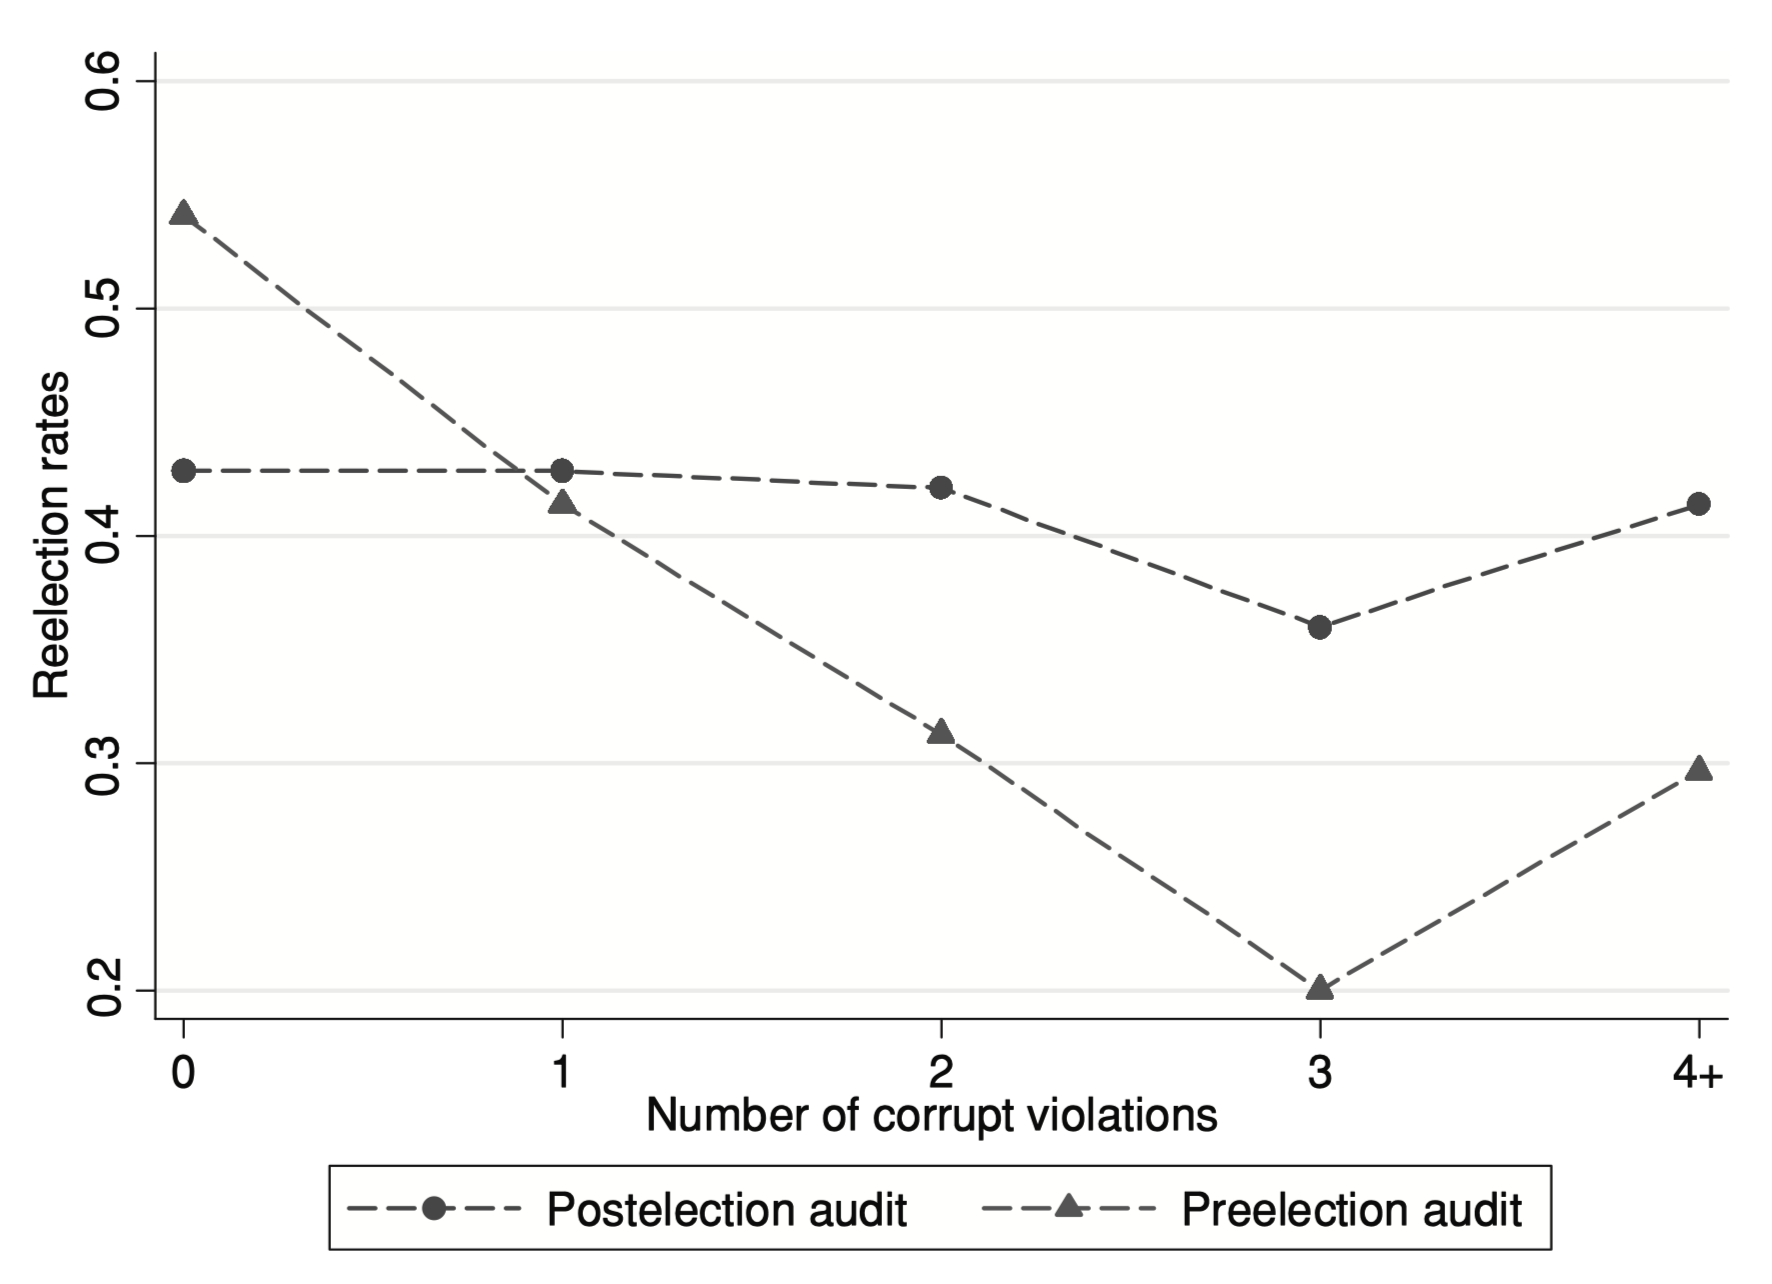
\includegraphics[height = 0.55 \textheight]{images/fig3.png}
            \end{figure}
        \end{column}

        \begin{column}{0.55\textwidth}

            \only<2->{
                \begin{table}[h!]
                    \footnotesize
                    \begin{center}
                        \label{tab:result2-1}
                        \begin{tabular}{lcc}
                        
                        \multicolumn{3}{c}{\color{orange}Linear}\\
                        & (1) & (2) \\
                        \hline
                        Preelection audit $\times$ & -0.038 & -0.038 \\
                         No. corruption violations & (0.035) & (0.035) \\
                         & \\
                         Observations & 373 & 373 \\
                         $R^2$ & 0.05 & 0.18\\
                         State FEs & Yes & Yes\\
                         Municipal controls & \textcolor{orange}{No} & \textcolor{orange}{Yes} \\
                         Mayoral controls & \textcolor{orange}{No} & \textcolor{orange}{Yes} 
                        \end{tabular}
                    \end{center}
                    \end{table}
            }
        
        \end{column}

    \end{columns}

\end{frame}

\begin{frame}{Estimation II: Adding Voters' Prior Beliefs}

    \begin{columns}

        \begin{column}{0.4\textwidth}
            \begin{figure}
            \centering
            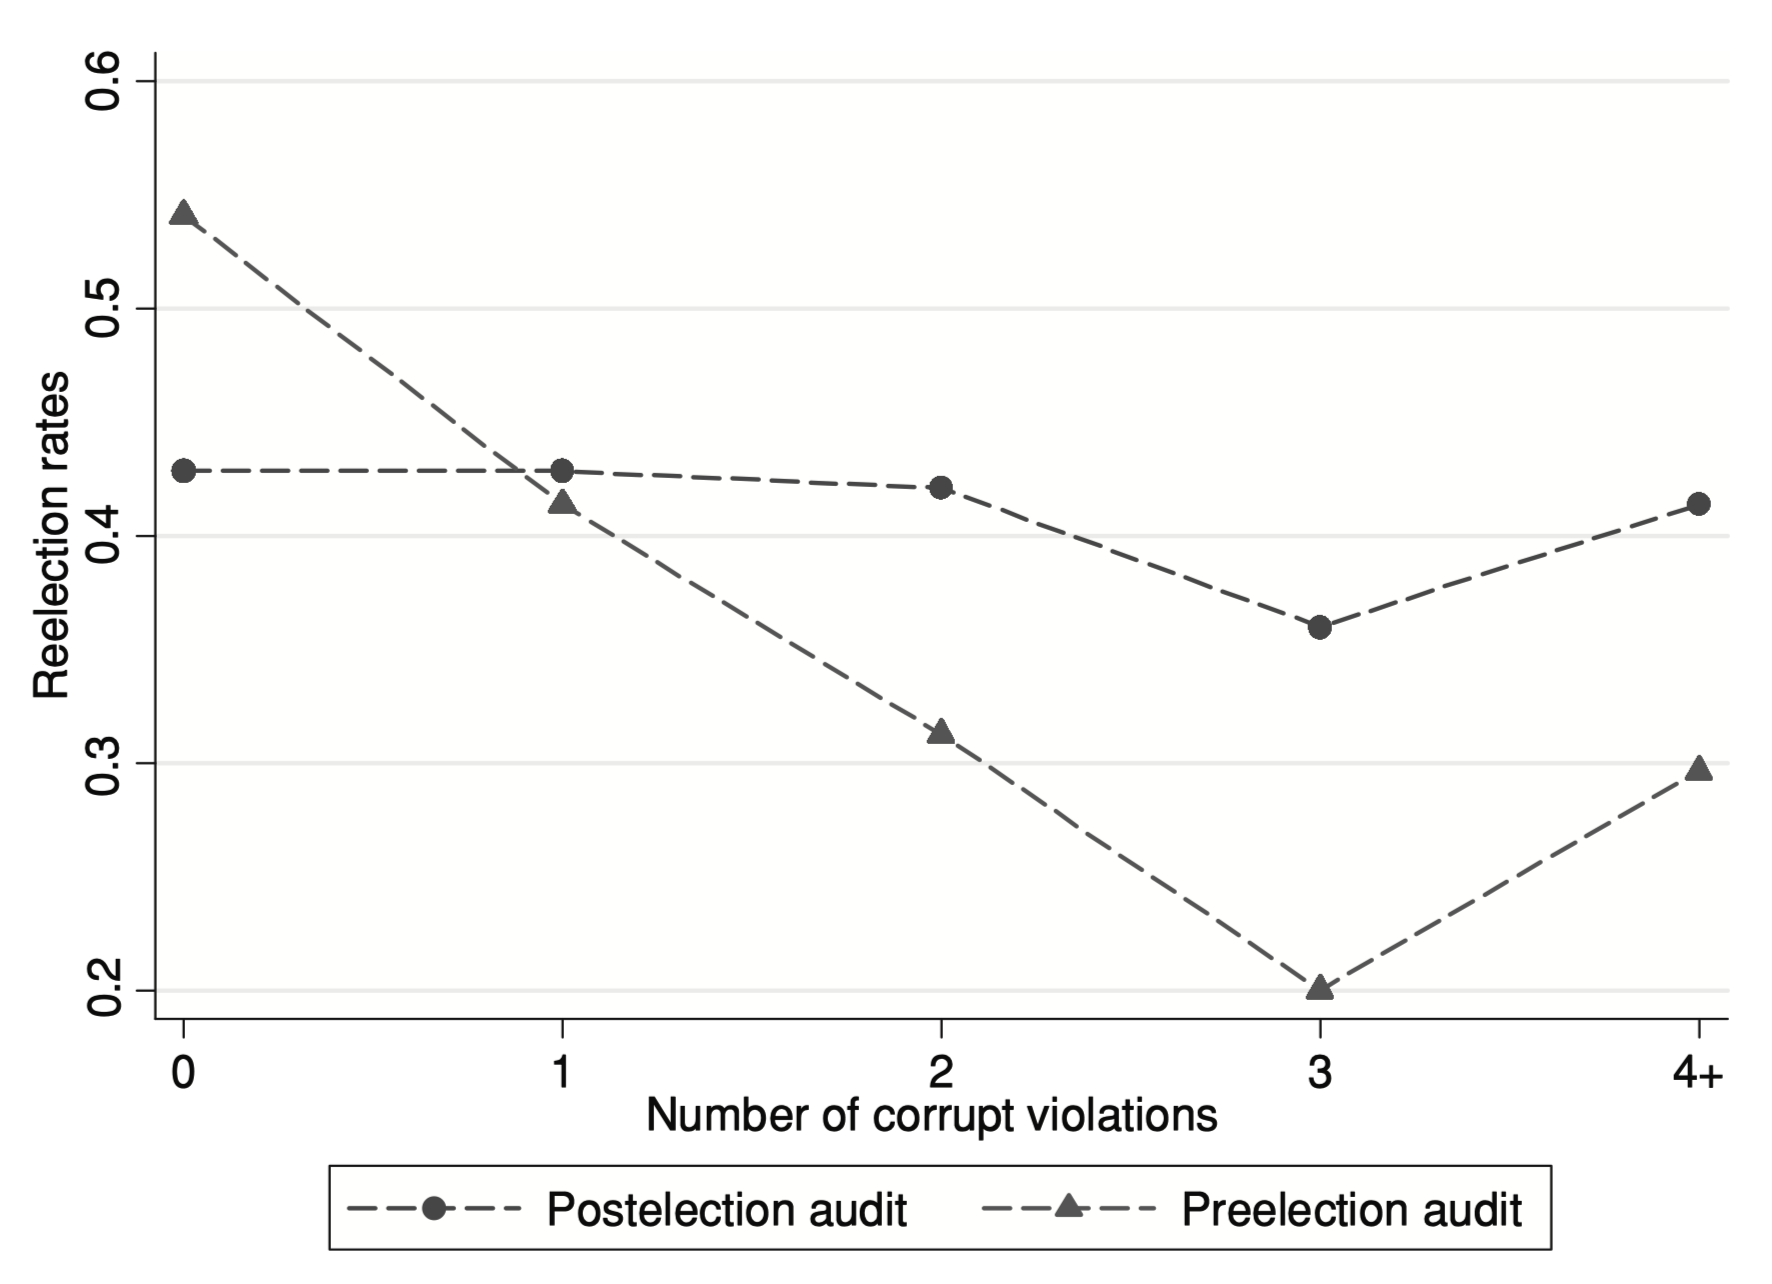
\includegraphics[height = 0.55 \textheight]{images/fig3.png}
            \end{figure}
        \end{column}

        \begin{column}{0.55\textwidth}

            \only<1->{
                \begin{table}[h!]
                    \tiny
                    \begin{center}
                        \label{tab:result2-2}
                        \begin{tabular}{lccc}
                        
                        \multicolumn{4}{c}{Different models}\\
                        \hline
                        & Linear & \textcolor<2>{orange}{Quadratic} & \textcolor<3>{orange}{Semiparametric} \\
                        & (2) & (3) & (4)\\
                        \hline
                        Preelection audit $\times$ & -0.038 & \textcolor<2>{orange}{-0.200$^*$} & \\
                         No. corruption violations & (0.035) & (0.090) & \\
                         Preelection audit $\times$ &  & \textcolor<2>{orange}{0.034$^*$} &\\
                         No. corruption violations$^2$ & & (0.017) &\\
                         
                         Preelection audit $\times$ &  & & 0.010\\
                         corruption = 0 & & & (0.156)\\
                         Preelection audit $\times$ &  & &  \textcolor<3>{orange}{-0.253$^+$}\\
                         corruption = 2 & & & (0.148)\\
                         Preelection audit $\times$ &  &  & \textcolor<3>{orange}{-0.321$^+$}\\
                         corruption = 3 & & & (0.192)\\
                         Preelection audit $\times$ &  &  & -0.159\\
                         corruption = 4 & & & (0.168)\\
                         & \\
                         $R^2$ & 0.18 & \textcolor<2>{orange}{0.19} & \textcolor<3>{orange}{0.22} \\
                         $F-$test ($p$-value) & & \textcolor<2>{orange}{0.089} & \textcolor<3>{orange}{0.192}
                        \end{tabular}
                    \end{center}
                    \end{table}
            
            }
        
        \end{column}

    \end{columns}

\end{frame}

\begin{frame}{Estimation II: Adding Voters' Prior Beliefs}

    \begin{columns}

        \begin{column}{0.4\textwidth}
            \begin{figure}
            \centering
            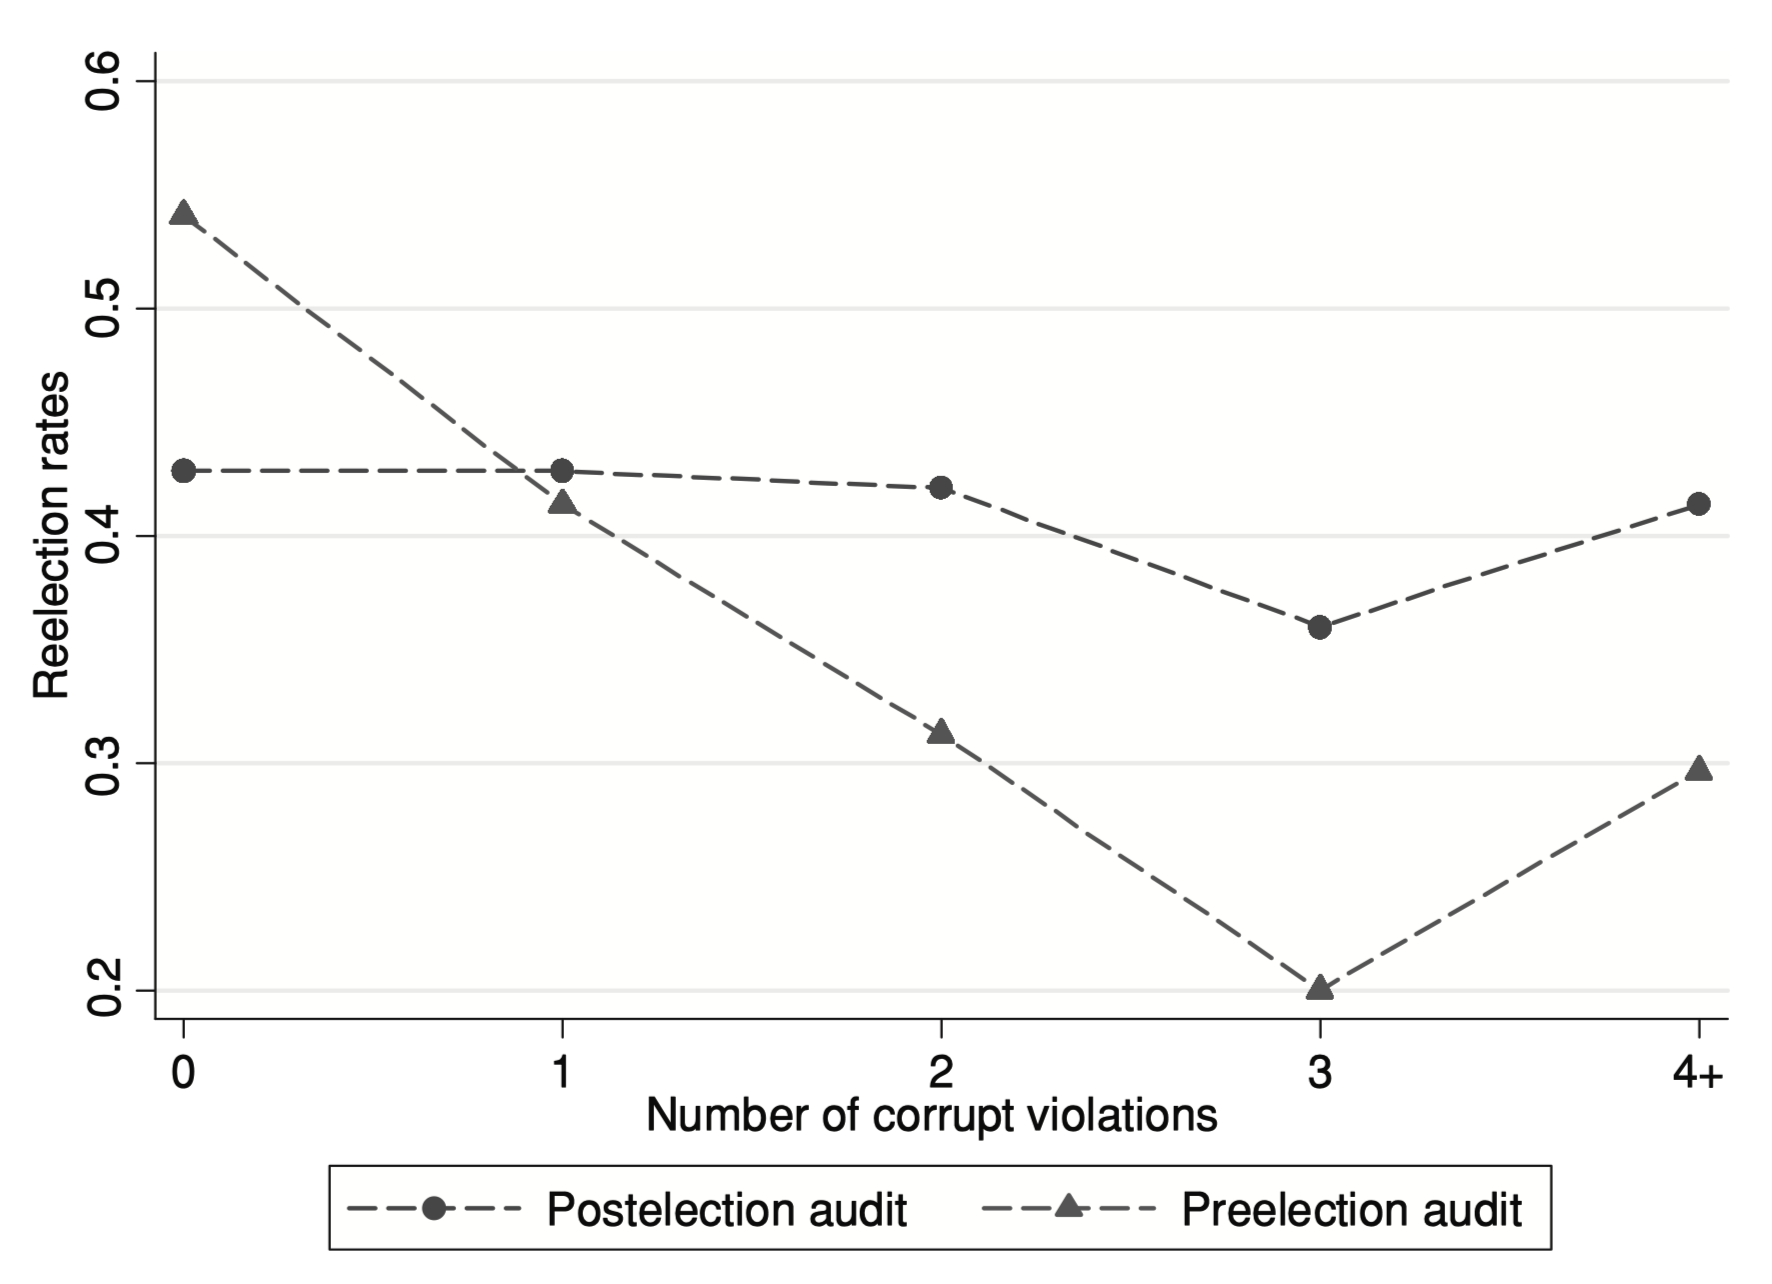
\includegraphics[height = 0.55 \textheight]{images/fig3.png}
            \end{figure}
        \end{column}

        \begin{column}{0.55\textwidth}

            \only<1->{
                \begin{table}[h!]
                    \tiny
                    \begin{center}
                        \label{tab:result2-3}
                        \begin{tabular}{lccc}
                        
                        \multicolumn{4}{c}{Different samples}\\
                        \hline
                        & Full & \textcolor<2>{orange}{Corruption$\leq$5} & \textcolor<3>{orange}{Corruption$\leq$4} \\
                        & (2) & (5) & (6)\\
                        \hline
                        Preelection audit $\times$ & -0.038 & \textcolor<2>{orange}{-0.070$^+$} & \textcolor<3>{orange}{-0.088$^*$} \\
                         No. corruption violations & (0.035) & (0.041) & (0.043)\\
                         & \\
                         Observations & 373 & \textcolor<2>{orange}{362} & \textcolor<3>{orange}{351} \\
                         $R^2$ & 0.18 & 0.19 & 0.20
                        \end{tabular}
                    \end{center}
                    \end{table} 
            
            }
        
        \end{column}

    \end{columns}

\end{frame}

\begin{frame}{Estimation II: Adding Voters' Prior Beliefs}

    \begin{columns}

        \begin{column}{0.4\textwidth}
            \begin{figure}
            \centering
            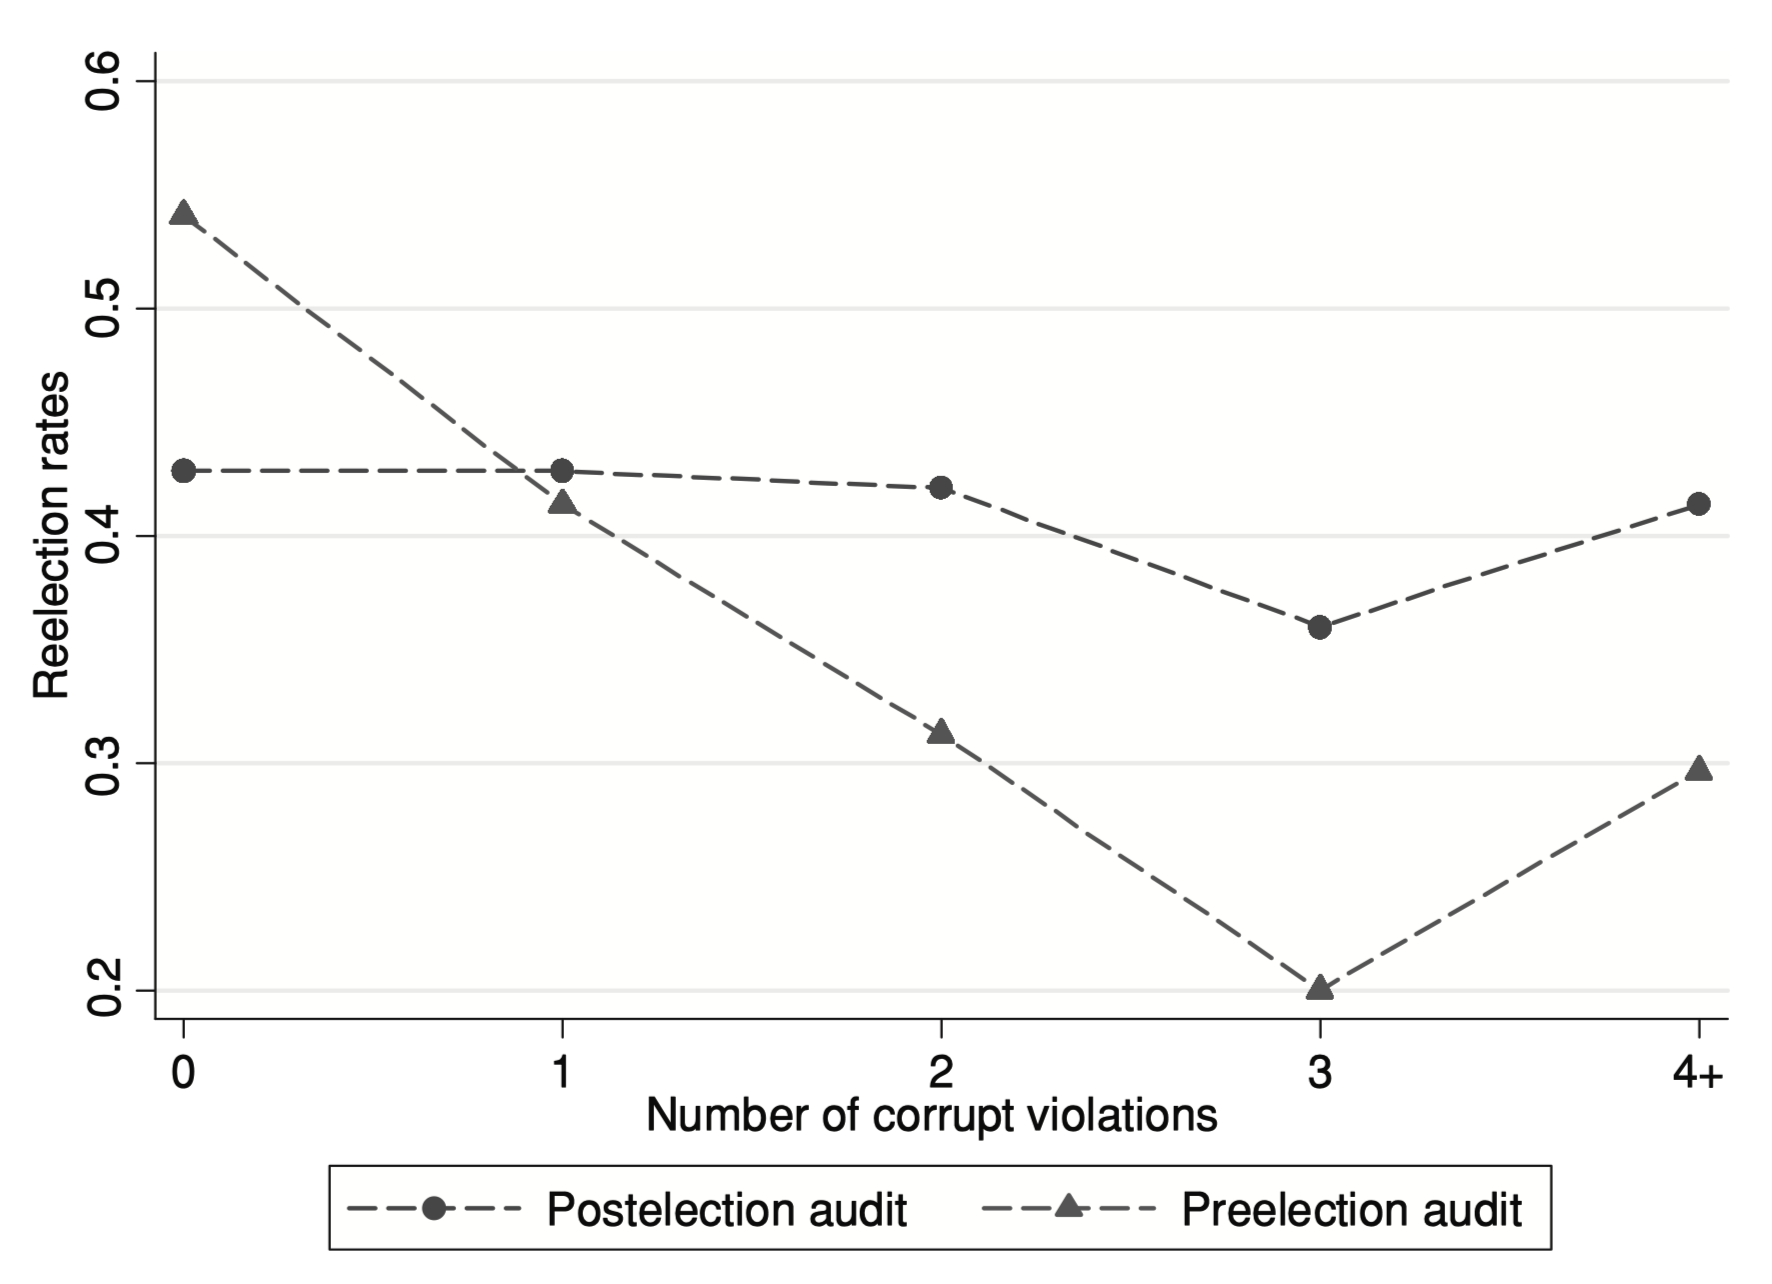
\includegraphics[height = 0.55 \textheight]{images/fig3.png}
            \end{figure}
        \end{column}

        \begin{column}{0.5\textwidth}

        \only<1->{
        \begin{block}{\small \textbf{Summary}}
        \footnotesize

            \only<1->{
                \begin{enumerate}
                    \item<2-> Model selection: The U-shape relationship is more likely driven by \textbf{\color{orange}noise}
                    \item<3-> Preferred specification: \textbf{\color{orange} Linear}, with the sub-sample of \textbf{\color{orange}Corruption$\leq$5} 
                    \item<4-> Estimation results: Marginal treatment effect per corruption violation is \textbf{\color{orange}-7\%} {\scriptsize (or \textbf{\color{orange}-16\%} of the 43\% control-group reelection rate)}.
                    \item<5-> Prior belief: Incumbents on average commit \textbf{\color{orange}1} corrupt violation 
                \end{enumerate}
            }
        \end{block}
        }

        \only<6>{\scriptsize
            \textbf{\color{orange}Question}: what about those extremely corrupted mayors?
        }
        
        \end{column}

    \end{columns}

\end{frame}


\begin{frame}{Estimation III: Adding the Presence of Local Media}
    \only<1->{
        \tiny
        \begin{align*}
        E_{ms} =& \alpha + \beta_0C_{ms} + \beta_1 A_{ms} + \textcolor<5>{orange}{\beta_2} M_{ms} + \textcolor<3>{orange}{\beta_3} \left(A_{ms}\times M_{ms}\right) + \beta_4\left(A_{ms}\times C_{ms}\right)\\
        & + \textcolor<4>{orange}{\beta_5} \left(M_{ms}\times C_{ms}\right) + \textcolor<2>{orange}{\beta_6} \left( A_{ms}\times C_{ms}\times M_{ms} \right) + X_{ms}\gamma+\nu_s +\epsilon_{ms}
        \end{align*}
    }

    \only<1->{
        \begin{table}[h!]
            \scriptsize
            \begin{center}
                \label{tab:result3-1}
                \begin{tabular}{lcccc}
                
                %\multicolumn{5}{c}{Dependent variable: Pr(reelection)}\\
                %\hline
                & & & & Demographics\\
                & Full & Corruption$\leq$5 & Demographics &  \& institutional  \\
                & (1) & (2) & (3) & (4) \\
                \hline
                 Preelection audit & -0.059 & -0.033 & 0.296 & 0.208 \\
                 No. corrupt violations & -0.034 & -0.013 & -0.13 & -0.069\\
                 No. radio stations & \textcolor<5>{orange}{-0.131$^*$} & \textcolor<5>{orange}{-0.150$^*$} & \textcolor<5>{orange}{-0.216$^{**}$} & \textcolor<5>{orange}{-0.253$^{**}$}\\
                 &\\
                 Preelection audit $\times$ No. radio stations & \textcolor<3>{orange}{0.229$^*$} & \textcolor<3>{orange}{0.271$^{**}$} & \textcolor<3>{orange}{0.356$^{**}$} & \textcolor<3>{orange}{0.449$^{**}$} \\
                 Preelection audit $\times$ No. corrupt violations & 0.007 & -0.018 & -0.236 & -0.412 \\
                 No. radio stations $\times$ No. corrupt violations & \textcolor<4>{orange}{0.050$^{+}$} & \textcolor<4>{orange}{0.058$^*$} & \textcolor<4>{orange}{0.082$^{**}$} &\textcolor<4>{orange}{0.09$^{**}$}\\
                 &\\
                 Triple interaction & \textcolor<2>{orange}{-0.118$^{**}$} & \textcolor<2>{orange}{-0.157$^*$} & \textcolor<2>{orange}{-0.185$^{**}$} & \textcolor<2>{orange}{-0.238$^{**}$}\\
                 &\\
                 $R^2$ & 0.20 &0.21 & 0.24 & 0.28
                \end{tabular}
            \end{center}
            \end{table}
    }

    
\end{frame}

\begin{frame}{Estimation III: Adding the Presence of Local Media}

    \begin{columns}

        \begin{column}{0.5\textwidth}
            \begin{figure}
            \centering
            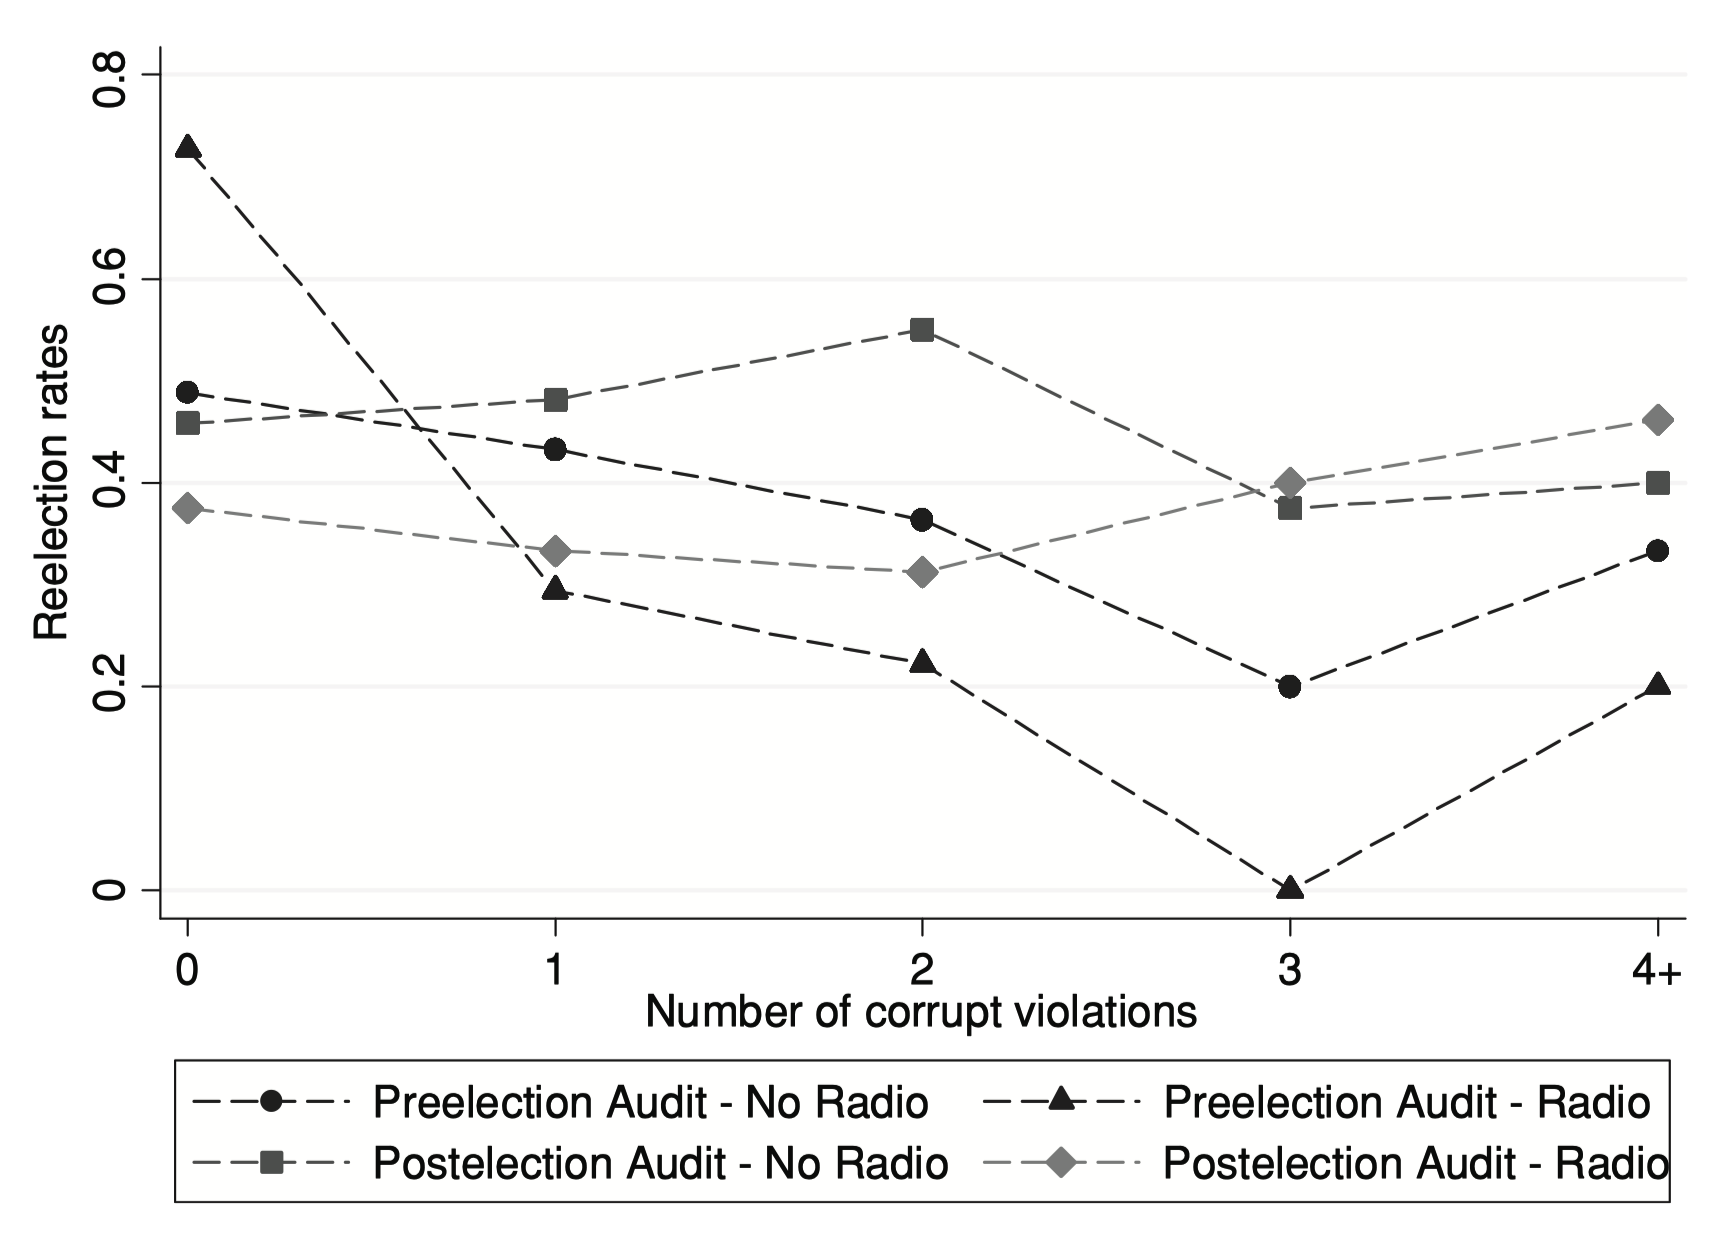
\includegraphics[height = 0.65 \textheight]{images/fig4.png}
            \end{figure}
        \end{column}

        \begin{column}{0.5\textwidth}

            \only<1->{
                \scriptsize
                \begin{align*}
                E_{ms} = & \alpha + \beta_0C_{ms} + \beta_1 A_{ms} + \textcolor{orange}{\beta_2} M_{ms} \\
                & + \textcolor{orange}{\beta_3} \left(A_{ms}\times M_{ms}\right) + \textcolor{orange}{\beta_5}\left(M_{ms}\times C_{ms}\right)\\
                & + \beta_4\left(A_{ms}\times C_{ms}\right) \\
                & + \textcolor{orange}{\beta_6} \left( A_{ms}\times C_{ms}\times M_{ms} \right) + X_{ms}\gamma+\nu_s +\epsilon_{ms}
                \end{align*}
            }

            \only<2->{
                \begin{itemize}
                    \item<2-> \textcolor{orange}{$\beta_6<0$}
                    \item<3-> \textcolor{orange}{$\beta_5>0$}, $\beta_4=0$, \textcolor{orange}{$\beta_3>0$}
                    \item<4-> \textcolor{orange}{$\beta_2<0$}, $\beta_1=0$, $\beta_0=0$ 
                \end{itemize}
            }

        
        \end{column}

    \end{columns}

\end{frame}

    \section{Discussion}
    
    \frame{\sectionpage}
    
    \begin{frame}{\textit{Robustness check:} Concerns addressed}

        \begin{enumerate}
            \item<2-> Audit process manipulation
            \only<2->{
                \begin{itemize}
                    \item<3-> Control for \textbf{\color{orange}corrupted auditors}: state fixed effects {\scriptsize (Q: standard error)}
                    \item<4-> Control for mayors' \textbf{\color{orange}political power}: party information {\scriptsize (Table V Column 1-4)}
                    \item<5-> Control for mayors' idiosyncratic \textbf{\color{orange}incentives to bribe}: narrow win for 1st term in 2000 {\scriptsize (Table V Column 2-4)}
                \end{itemize}
            }
            \item<6-> Dynamic: early audit treatments induce a learning effect
            \begin{itemize}
                \item<7-> Re-estimate on sub-samples of \textbf{\color{orange}different time windows} {\scriptsize (Table V Column 5-6)}
            \end{itemize}

            \item<8-> Placebo test: the audit treatment is not correlated with 2000 election results.
            
        \end{enumerate}
    
    \end{frame}

    \begin{frame}{\textit{Robustness check:} Concerns addressed}

        \begin{enumerate}
            \item<1-> Media availability: Is it just a proxy?
            \begin{itemize}
                \item<2-> \textbf{\color{orange}eduation level}: audit information is better received/interpreted, educated citizens are more politically engaged
                \item<3-> \textbf{\color{orange}polulation size}: political scandals travel faster in the bigger crowd
                \item<4-> \textbf{\color{orange}economic diversity}: audit information is not so important in municipalities with high income inequality
            \end{itemize}

            \only<5->{Control for these factors, the effect of media presence is stable and significant.}

            \item<6-> Different measures of electoral outcomes and media presence
        \end{enumerate}
    
    \end{frame}
    
    \begin{frame}{What are other concerns?}
        \begin{enumerate}
            \item<1-> Voters' behavior (partially addressed):
            \only<2->{
                \begin{itemize}
                    \item[-] Heterogeneity in beliefs and the formation of beliefs
                    \item[-] How voters think about and react to corruption
                    \item[-] Asymmetry of punishment and reward after the \textit{shock}
                \end{itemize}
            }
            \item<3-> Spillover effects (partially addressed):
            \only<4->{
                \begin{itemize}
                    \item[-] Between politicians
                    \item[-] Between municipalities/individual voters
                    \item[-] Between auditor teams
                \end{itemize}
            }
            \item<5-> Long term effect for politicians seeking for higher positions
            \item<6-> Magnitude of corruption 
            \item<7-> Next-step consequences (reduction of corruption, studied in \citet{avis2018government})
        \end{enumerate}

    \end{frame}

    \begin{frame}{Final Comments}
        \begin{columns}[T]

            \begin{column}{0.4\textwidth}
                \begin{block}{\small \textbf{What I like...}}
                \footnotesize
                    \only<1->{\begin{itemize}
                        \item<1-> empirical completeness
                        \item<2-> a \textit{clean} study
                        \item<3-> good attempt on revealing the mechanism behind
                    \end{itemize}}
                \end{block}
            \end{column}
            
            \begin{column}{0.4\textwidth}
            
            \only<1->{
            \begin{block}{\small \textbf{What I don't like}}
            \footnotesize
               \only<1->{\begin{itemize}
                   \item<4-> \textit{too} reduced-form
                   \item<5-> \textit{so} much anecdotal evidence that it becomes un-informative
                   \item<6-> TYPOS, in tables :(
               \end{itemize}}
            \end{block}
            }
            
            \end{column}
            \end{columns}
    \end{frame}

\section*{References}
\begin{frame}[allowframebreaks]{References}
    \printbibliography[heading=none]
\end{frame}
    
\part{}
    \begin{frame}[plain,c]
    \begin{center}
       \Huge
        \textcolor{frenchlilac}{Thank you!} 
        
    \end{center}
    \end{frame}
\end{document}
